\section{Análise}

A leitura de \textit{O Pássaro}, de Augusto Frederico Schmidt, será orientada
principalmente pela narrativa da Criação presente no livro de Gênesis.

Para as citações bíblicas, será utilizada a tradução do \textbf{Pe. Antônio
Pereira de Figueiredo}, baseada na Vulgata Latina \cite{figueiredo1794}. A
versão consultada está disponível gratuitamente em sua edição digital
\cite{bibliatraduzida_figueiredo}. A Figura~\ref{fig:biblia-familiar} apresenta
o exemplar físico utilizado como referência nesta análise.

\begin{figure}[ht]
  \centering
  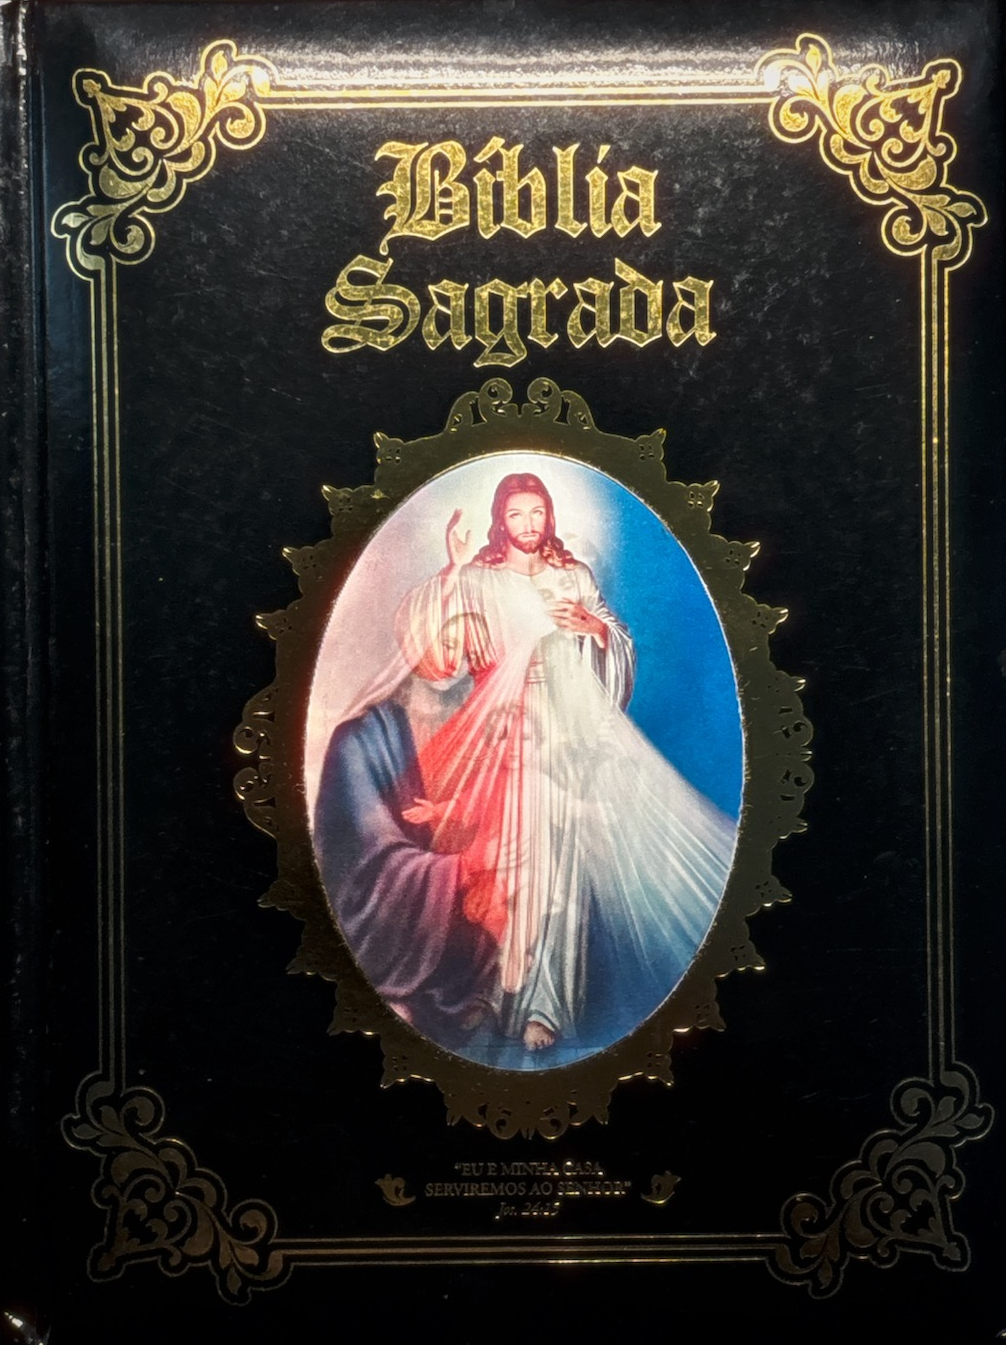
\includegraphics[width=0.45\textwidth]{./fig/Biblia-Familiar.png}
  \caption{Exemplar físico da Bíblia Sagrada utilizada como referência.}
  \label{fig:biblia-familiar}
\end{figure}

O poema constrói uma sequência de imagens que permite essa aproximação: a
``noite imóvel'', as trevas, as águas, o surgimento da luz, o movimento das
criaturas e, finalmente, a inauguração do tempo. A partir desses elementos,
podemos observar como o poema transforma poeticamente motivos associados ao
relato da Criação.

Em Gênesis, a narrativa começa em um cenário marcado pela escuridão, pelas
águas e pela ausência de uma ordem já estabelecida:

\begin{biblequote}[0.6\textwidth][1]{Genesis 1:1--2}
\bibleverse{No princípio criou Deus o céu e a terra.}
\bibleverse{A terra, porém, estava vazia e nua; e as trevas cobriam a face do
abismo; e o espírito de Deus era levado por cima das águas.}
\end{biblequote}

A imagem da terra ``vazia e nua'', juntamente com as ``trevas'' que cobrem o
``abismo'', estabelece um estado anterior à ordenação do mundo. O início de
\textit{O Pássaro} recupera justamente essa atmosfera primordial, substituindo
o ``abismo'' bíblico pela ``noite imóvel'':

\begin{poemquote}[0.49\textwidth]{1}
O pássaro estremece a noite imóvel \\
Com suas asas.
\end{poemquote}

A palavra ``imóvel'' é particularmente significativa. Ela não indica apenas a
ausência de movimento físico, mas pode sugerir um estado anterior ao próprio
desencadeamento da ordem e do tempo. Nesse sentido, a imagem permite uma
aproximação, ainda que não uma identificação direta, com o conceito
aristotélico de \textbf{Motor Imóvel}: aquilo que, não sendo movido por outro,
constitui o princípio último do movimento. Essa concepção seria posteriormente
retomada e desenvolvida por \textbf{Santo Tomás de Aquino}, especialmente em
sua reflexão sobre as vias para a demonstração da existência de Deus.

É justamente essa relação entre \textbf{imobilidade e movimento} que torna a
aproximação anterior particularmente sugestiva. O poema parte da ``noite
imóvel'' para introduzir imediatamente um movimento: o pássaro a ``estremece''
com suas asas. A imobilidade, portanto, constitui o estado a partir do qual o
movimento se manifesta. Não se trata, evidentemente, de afirmar que o pássaro
corresponda ao Motor Imóvel aristotélico; a aproximação está na estrutura da
imagem: assim como o conceito filosófico procura explicar o movimento a partir
de um princípio que não é movido, o poema constrói sua cena inaugural a partir
de uma imobilidade que é rompida pelo primeiro movimento. A oposição entre
``imóvel'' e ``estremece'' estabelece, assim, a passagem fundamental do poema:
da imobilidade primordial surge o movimento, e desse movimento começará a
surgir a vida.

Essa leitura também prepara a afirmação imediatamente posterior de que o
pássaro é ``o primeiro sinal de vida'': sua aparição não é apenas a entrada de
um animal em uma paisagem já existente, mas o primeiro movimento que rompe o
silêncio e a imobilidade da cena primordial.

\begin{poemquote}[0.49\textwidth]{3}
O pássaro é o primeiro sinal de vida. \\
É o primeiro som molhando o espaço.
\end{poemquote}

A expressão ``primeiro sinal de vida'' possui forte valor cosmogônico. O
pássaro não é apresentado simplesmente como uma criatura que já existe em um
mundo formado. Ele aparece \textbf{no instante em que o mundo começa a adquirir
vida}. Há, portanto, uma inversão em relação à ordem literal de Gênesis:
enquanto o relato bíblico apresenta primeiro a organização da criação e somente
posteriormente a criação das aves, o poema faz do pássaro o próprio anúncio do
despertar do mundo.

Além disso, o ``som'' do pássaro pode ser colocado em paralelo com a dimensão
sonora da criação bíblica. Em Gênesis, a fórmula criadora é repetidamente
introduzida pela palavra divina: ``Disse Deus''. A criação acontece mediante a
palavra. Em Schmidt, por sua vez, o primeiro som que rompe o silêncio é o do
pássaro. O canto ou movimento sonoro da ave adquire, assim, uma função quase
\textbf{verbal e criadora}: ele anuncia que a realidade está deixando de ser
silenciosa e imóvel.

A relação com o primeiro dia da Criação torna-se particularmente clara no
surgimento das luzes:

\begin{poemquote}[0.49\textwidth]{5}
Abre-se na superfície escura uma leve ferida, \\
Por onde começam a surgir luzes virgens,
\end{poemquote}

Em Gênesis, Deus ordena:

\begin{biblequote}[0.6\textwidth][3]{Genesis 1:3}
\bibleverse{Disse Deus: Faça-se a luz; e fêz-se a luz.}
\end{biblequote}

Nos dois textos, portanto, a luz nasce a partir de uma realidade inicialmente
dominada pela escuridão. Entretanto, Schmidt substitui a ação direta da palavra
divina por uma imagem de \textbf{abertura}. A ``superfície escura'' sofre uma
``leve ferida'', através da qual as luzes começam a surgir.

A escolha da palavra ``ferida'' é carregada de significado. Uma ferida
normalmente implica ruptura da integridade de uma superfície. Aqui, porém, a
ruptura é necessária para que a luz possa aparecer. A criação é representada
como uma \textbf{ruptura da escuridão}. A imagem pode ser entendida como uma
tradução poética da separação entre luz e trevas presente em Gênesis: a ordem
surge porque aquilo que estava fechado é rompido e delimitado.

O adjetivo ``virgens'', aplicado às luzes, reforça ainda mais a ideia de
criação. São luzes que aparecem como algo absolutamente novo, ainda não
experimentado. O poema não descreve simplesmente o nascer do dia; ele produz a
sensação de que \textbf{o próprio primeiro dia está sendo criado diante do
leitor}.

Essa leitura é reforçada pela maneira como as luzes se transformam:

\begin{poemquote}[0.49\textwidth]{7}
Que logo se enfloram, \\
E no espaço, vigorosas e jovens, se atiram.
\end{poemquote}

O vocabulário utilizado sugere crescimento e expansão. ``Enfloram'',
`vigorosas'', ``jovens'' e ``se atiram'' constituem um campo semântico de
nascimento, juventude e movimento. A criação não é apresentada como um
acontecimento estático, mas como um processo de \textbf{expansão da vida pelo
espaço}.

Nesse ponto, o poema também se aproxima do terceiro dia de Gênesis, quando Deus
ordena que a terra produza vegetação e árvores frutíferas, cada uma contendo em
si mesma a sua semente para a reprodução:

\begin{biblequote}[0.6\textwidth][11]{Genesis 1:11--13}
\bibleverse{Disse também Deus: Produza a terra erva verde, que dê a sua
semente; e produza árvores frutíferas, que deem fruto, segundo a sua espécie, e
que contenham a sua semente em si mesmas, para a reproduzirem sôbre a terra. E
assim se fêz.}
\bibleverse{E produziu a terra erva verde, que dava semente segundo a sua
espécie; e produziu árvores frutíferas que continham a sua semente em si
mesmas. E viu Deus que isto era bom.}
\bibleverse{E da tarde e da manhã se fêz o dia terceiro.}
\end{biblequote}

A relação com o poema torna-se especialmente evidente no verbo ``frutificará'',
empregado por Schmidt em seu encerramento. Assim como, no relato bíblico, o
fruto contém em si a semente que permite a reprodução, o pássaro que
``frutificará'' não representa apenas uma vida que surge, mas uma vida que
possui em si mesma a possibilidade de continuidade. O verbo ``frutificar''
desloca, portanto, para o pássaro uma imagem originalmente associada à
fecundidade da terra: aquilo que nasce não permanece isolado nem se encerra no
instante de sua aparição, mas participa de um processo contínuo de geração.
Essa ideia torna-se ainda mais significativa quando o poema projeta essa
frutificação para a ``eternidade prometida'', fazendo da vida inaugurada pelo
pássaro não apenas um acontecimento inicial, mas uma realidade destinada à
permanência.

As ``luzes'' apresentam ainda uma transformação expressiva, que pode ser
aproximada da criação dos luzeiros no quarto dia de Gênesis.

\begin{biblequote}[0.6\textwidth][11]{Genesis 1:11--13}
\bibleverse{Disse também Deus: Façam-se uns luzeiros no firmamento do céu, que
dividam o dia e a noite, e sirvam de sinais nos tempos, as estações, os dias e
os anos;que luzam no firmamento do céu, e alumiem a terra. E assim se fêz.}
\bibleverse{Fêz Deus, pois, dois grandes luzeiros, um maior, que presidisse ao
dia; outro mais pequeno, que presidisse à noite: e criou também as estrêlas. e
pô-las no firmamento do céu para luzirem sôbre a terra, e presidirem ao dia e à
noite, e dividirem a luz, das trevas. E viu Deus que isto era bom.}
\bibleverse{E da tarde, e da manhã se fêz o dia quarto.}
\end{biblequote}

Depois de separar a luz das trevas, Deus estabelece no firmamento os luzeiros
destinados a iluminar a terra e a ``dividir o dia e a noite'', servindo também
``de sinais nos tempos, as estações, os dias e os anos'':

\begin{poemquote}[0.49\textwidth]{9}
São luzes frescas, que têm a forma inicial \\
De lágrimas deslizando na face da sombra, \\
Mas que nos campos celestes, \\
Soltas e livres, tomam as formas de corcéis.
\end{poemquote}

Aqui, o poema transforma progressivamente a imagem da criação. Primeiro, as
luzes são ``lágrimas'' sobre a ``face da sombra''; depois, tornam-se
``corcéis'' nos ``campos celestes''. O termo ``corcel'' designa um
\textbf{cavalo veloz}, especialmente um cavalo de batalha ou de grande vigor,
como na expressão ``fogoso corcel''. A escolha dessa palavra, portanto,
acrescenta à imagem das luzes as ideias de \textbf{velocidade, força e
movimento}. A passagem da lágrima ao corcel representa, assim, uma
transformação da \textbf{fragilidade em força e liberdade}: aquilo que
inicialmente escorre suavemente pela ``face da sombra'' passa a mover-se
vigorosamente pelos ``campos celestes''.

O espaço celeste também pode ser relacionado ao firmamento de Gênesis. Depois
de separar luz e trevas, o relato bíblico apresenta a criação do firmamento,
que divide as águas e recebe os luzeiros. O poema não reproduz essa sequência
literalmente, mas conserva sua estrutura imagética: existe uma superfície
inicialmente escura, surgem luzes e, em seguida, essas luzes ocupam um espaço
celeste aberto.

A presença do ``mar'' torna a relação com Gênesis ainda mais explícita:

\begin{poemquote}[0.49\textwidth]{13}
O pássaro paira sobre o mar recém-nascido \\
E inaugura o tempo.
\end{poemquote}

O verbo ``paira'' retoma, de modo indireto, a imagem do espírito de Deus que se
move sobre as águas no início de Gênesis. No poema, porém, é o pássaro que
ocupa essa posição, pairando sobre o ``mar recém-nascido''. A escolha do verbo
é significativa porque suspende o movimento do pássaro entre o voo e o repouso:
ele não atravessa simplesmente o espaço, mas permanece sobre a paisagem que
acaba de surgir. A imagem confere ao pássaro uma posição liminar, entre o céu e
o mar, justamente no momento em que o poema passa da criação do espaço à
inauguração do tempo.

Essa aproximação ganha uma dimensão ainda mais interessante quando se observa a
posição das aves na narrativa de Gênesis. Elas são criadas somente no quinto
dia, depois da separação das águas e da criação dos luzeiros:

\begin{biblequote}[0.6\textwidth][20]{Genesis 1:20}
\bibleverse{Disse também Deus: Produzam as águas animais viventes, que nadem
nas águas; e aves, que voem sôbre a terra, e debaixo do firmamento do céu.}
\end{biblequote}

Schmidt desloca, portanto, a ave para o próprio momento inaugural da paisagem.
Ela não aparece como parte de um mundo já ordenado, mas sobre um ``mar
recém-nascido'', antes que a criação esteja plenamente constituída. O pássaro
assume, assim, uma posição que antecede simbolicamente aquela que lhe é
atribuída no relato bíblico.

Essa antecipação prepara o verso ``E inaugura o tempo''. Em Gênesis, a
temporalidade da criação é estabelecida pela sucessão de ``tarde'' e ``manhã'',
a partir do primeiro dia. No poema, essa ideia é condensada no verbo
``inaugura'': o pássaro não apenas surge dentro do tempo, mas aparece no limiar
de sua constituição. O movimento iniciado na noite imóvel alcança, nesse ponto,
uma dimensão temporal: a paisagem deixa de ser apenas espaço e passa a possuir
uma ordem de acontecimentos.

O final do poema amplia essa temporalidade para além de seu próprio início:

\begin{poemquote}[0.49\textwidth]{15}
E frutificará \\
Na eternidade prometida.
\end{poemquote}

A ``eternidade'' desloca o poema da temporalidade recém-inaugurada para aquilo
que a transcende. O pássaro passa, assim, do instante inaugural à promessa de
permanência, encerrando o movimento do poema não com o fim do tempo, mas com a
sua superação.

A trajetória construída pelo poema pode ser compreendida como uma passagem
progressiva da \textbf{imobilidade à eternidade}:

\[
\text{imobilidade}
\longrightarrow
\text{movimento}
\longrightarrow
\text{manifestação}
\longrightarrow
\text{ordenação}
\longrightarrow
\text{tempo}
\longrightarrow
\text{eternidade}.
\]

Essa sequência aproxima \textit{O Pássaro} da estrutura cosmogônica de Gênesis,
sem fazer do poema uma simples paráfrase do texto bíblico. Schmidt retoma
imagens fundamentais da Criação --- as trevas, as águas, a luz, os luzeiros, as
aves e a ordenação do tempo --- e as reorganiza em torno da figura do pássaro.

Em Gênesis, a criação é ação direta de Deus, realizada por sua palavra. Em
Schmidt, não há uma figura divina nomeada; a transformação é construída pelas
imagens do poema, que conduzem da ``noite imóvel'' à ``eternidade prometida''.
O pássaro ocupa o centro dessa passagem, sem assumir propriamente o papel de
criador.

Sua trajetória acompanha as principais transformações do poema: rompe a
imobilidade inicial, acompanha o surgimento das luzes, paira sobre o ``mar
recém-nascido'' e ``inaugura o tempo''. No encerramento, o futuro de
``frutificará'' prolonga esse movimento para além do instante presente:

\begin{poemquote}[0.49\textwidth]{15}
E frutificará \\
Na eternidade prometida.
\end{poemquote}

A aproximação com Gênesis permite, assim, compreender \textit{O Pássaro} como
uma representação poética da origem e da continuidade da existência. O pássaro
concentra esse movimento ao atravessar as diferentes etapas da criação, da
imobilidade inicial à ``eternidade prometida''.
